\documentclass[../main.tex]{subfiles}

\begin{document}
\chapter{Derivatives}
\section{Geometric Interpretation}
\begin{figure}[h]
    \centering
    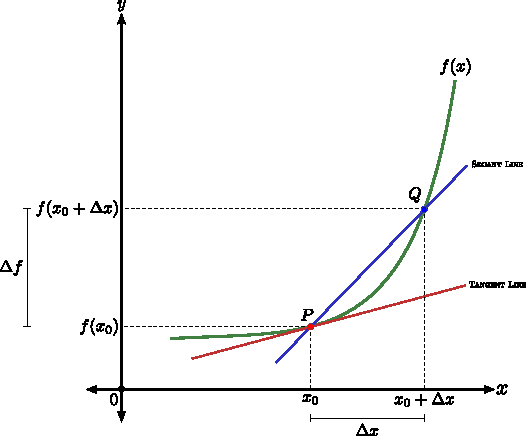
\includegraphics[width=\textwidth]{secant-tangent.pdf}
    \caption{A function with secant and tangent lines}
    \label{fig:secant-tangent}
\end{figure}
This is the graph of a function, $f(x)$, and $P$ and $Q$ are points
on that curve. Geometrically, the line $\overline{PQ}$ is known as the
\emph{secant} line --- a line that passes through at least two points
on a curve. We can see that the slope of $\overline{PQ}$ is 
$\frac{\Delta f}{\Delta x}$ and it is different than the slope ($m$) 
of the \emph{tangent} line.

\begin{defn}
    The derivative of $f$ at the point $x_0$, denoted $f'(x_0)$, is the
    slope of the tangent line to $y=f(x)$ at the point $P$.
    \label{def:derivative}
\end{defn}

Although that is a pretty solid definition of a derivative, 
we need to be careful about how we think about the tangent line. 
It is not just any line that passes through $P$; 
it is the \emph{limit} of the secant line as the distance between 
$P$ and $Q$ goes to $0$.

Similarly, the slope of $\overline{PQ}$ \emph{approaches} the slope of the 
tangent line as $Q \to P$. We can imagine this by dragging $Q$ 
along the path of the curve down to $P$ and think about how that would 
change the slope of $\overline{PQ}$. In the \emph{limiting} case, $Q$ 
would be right next to $P$ and the slope of $\overline{PQ}$ would be 
identical to the slope of the tangent line. 
This idea of limits is mathematically denoted in the following way:
\begin{equation}
    f' \left( x_0 \right) = \lim_{\Delta x \to 0} 
                                \frac
                                    {\Delta f}
                                    {\Delta x}
                          = \lim_{\Delta x \to 0}
                                \frac
                                    {
                                        f \left( x_0 + \Delta x \right)
                                        - f \left( x_0 \right)
                                    }
                                    {\Delta x}
                          = m
    \label{eqn:derivative}
\end{equation}

\begin{exmp}
    $f(x) = x^2$

    We need to find the general equation of the slope of the tangent line 
    at any point $x$ on the curve of $y=x^2$ in terms of $x$.

    From Equation \ref{eqn:derivative}, we have:
    \begin{equation*}
        f'(x) = \lim_{\Delta x \to 0}
                    \frac
                    {
                        f \left( x_0 + \Delta x \right)
                        - f \left( x_0 \right)
                    }
                    {\Delta x}
    \end{equation*}
    By plugging in the given function, we get:
    \begin{equation*}
        \begin{split}
            f'(x)   & = \lim_{\Delta x \to 0}
                            \frac
                            {\left( x + \Delta x \right)^2 - x^2}
                            {\Delta x}\\
                    & = \lim_{\Delta x \to 0}
                            \frac
                            {
                                x^2 +
                                2x \Delta x +
                                \left( \Delta x \right)^2 -
                                x^2
                            }
                            {\Delta x}\\
                    & = \lim_{\Delta x \to 0}
                            \frac
                            {\Delta x \left( 2x + \Delta x \right)}
                            {\Delta x}\\
                    & = \lim_{\Delta x \to 0} \left( 2x + \Delta x \right)\\
                    & = 2x
        \end{split}
    \label{eg:derivative}
    \end{equation*}
\end{exmp}
\subsection*{Notations}
Calculus, rather like English or any other language, 
was developed by several people. As a result, just as there are many ways 
to express the same thing in English, there are many notations for 
the derivative.

Since $y = f(x)$, it is natural to write:
\begin{equation*}
    \Delta y = \Delta f = f(x) - f \left( x_0 \right) =
    f \left( x_0 + \Delta x \right) - f \left( x_0 \right)
\end{equation*}
If we divide both sides by $\Delta x$, we get two expressions for
the \emph{difference quotient}:
\begin{equation*}
    \frac{\Delta y}{\Delta x} = \frac{\Delta f}{\Delta x}
\end{equation*}
As $\Delta x \to 0$:
\begin{align*}
    \frac{\Delta y}{\Delta x} & \to \left. \frac{dy}{dx} \right| _{x = x_0}
    & & \textrm{(Leibniz' Notation)}\\
    \frac{\Delta f}{\Delta x} & \to f' \left( x_0 \right)
    & & \textrm{(Newton's Notation)}\\
\end{align*}
Other, equally valid notations for the derivative of a 
function $f$ include:
\begin{equation*}
    f'(x) = f'  = Df = \frac{df}{dx} = \frac{dy}{dx} = \frac{d}{dx} y
          = \frac{d}{dx} f(x)
\end{equation*}
The \emph{dot notation} (also introduced by Newton) is another convention 
used to denote derivatives with respect to $t$:
\begin{equation*}
    \frac{dy}{dt} = \dot{y}
\end{equation*}
\subsection*{}
As we have seen from Example \ref{eg:derivative}, at any point $x$, the slope of the parabola, $x^2$, 
is $2x$. 
We can show that this can be generalised to the following formula:
\begin{equation}
    \frac{d}{dx} \left( x^n \right) = nx^{n - 1}
\end{equation}

\begin{exmp}
    \begin{align*}
        \frac{d}{dx} \left( x^3 + 3x^{10} \right)
            & = (3)x^{3-1} + 3(10)x^{10-1}\\
            & = 3x^2 + 30x^9
    \end{align*}
\end{exmp}
\section{Physical Interpretation}
When something is changing with respect some other thing, 
it can be useful to know fast it’s changing at a particular instant.

\begin{figure}[h]
    \centering
    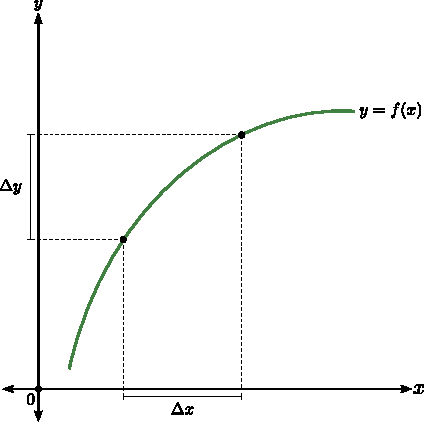
\includegraphics[width=0.75\textwidth]{average-change.pdf}
    \caption{Graph of a function with $\Delta x$ and $\Delta y$ labelled}
    \label{fig:average-change}
\end{figure}

Speed is a perfect example of this. When you are moving, the distance ($s$) 
you travel changes with time ($t$). The \emph{rate of change} of distance 
with respect to time (what we usually call \emph{speed}), 
is a measure of how fast you’re moving. Sometimes, it is useful to know 
what your \emph{average} speed ($\bar{v}$) was over the whole journey, 
which is given by:
\begin{equation*}
    \bar{v} = \frac{\Delta s}{\Delta t}
\end{equation*}
Other times, your speed at a particular instant is more important – 
this is what is known as your \emph{instantaneous} speed ($v$). 
You don’t get a speeding ticket for having a high average speed 
over the whole journey; you get one for having a high speed 
at the \emph{instant} you crossed a detection point. 
Similarly, the speed shown on a car’s speedometer is not your 
average speed for the whole trip, it is your instantaneous speed 
at that particular instant. Derivates do a great job at finding these 
instantaneous rates of change:
\begin{equation*}
    v = \frac{ds}{dt}
\end{equation*}
\begin{exmp}
    The distance ($s$) travelled by any free-falling object 
    over time ($t$) is, approximately:
    \[ s = 5t^2 \]
    In other words, after falling for one second, free-falling objects
    usually travel five meters. After two seconds, twenty meters, and so on.

    If we drop a ball from top of a five-hundred-meter tall building, 
    we know it will take about ten seconds to fall:
    \begin{align*}
        500 &= 5t^2\\
        \therefore t &= \SI{10}{s}
    \end{align*}
    Since we know $\Delta s = 500$ and $\Delta t = 10$, we can find 
    the average speed of the ball over its entire fall:
    \begin{align*}
        \bar{v} &= \frac{\Delta s}{\Delta t}\\
                &= \frac{500}{10}\\
                &= \SI{50}{m.s^{-1}}
    \end{align*}
    However, using differentiation, we can also find its 
    instantaneous speed at any instant during its ten-second fall. 
    We just need the derivative of $s$ with respect to $t$:
    \begin{align*}
        v   &= \frac{ds}{dt}\\
            &= \frac{d}{dt} \left( 5t^2 \right)\\
            &= 10t
    \end{align*}
    All we need to do now is plug in any value of $t$ we want, 
    and this derivative will tell us the speed of the ball at that 
    particular instant in time. After, say, six seconds of falling 
    ($t = \SI{6}{s}$), we know the ball was travelling at $v = \SI{60}{m.s^{-1}}$.
\end{exmp}
\end{document}